I valori di input, se non diversamente specificato, sono presi dal lavoro di \citet{DBLP:books/sp/Serazzi24}.

Le variabili indipendenti sono le seguenti:
\begin{itemize}
    \item Distribuzioni di probabilità dei servizi: Esponenziali;
    \item Distribuzioni di probabilità degli arrivi esterni: Esponenziali;
    \item Tempi di servizio medi per classe di job in ogni nodo: vedere \autoref{fig:average_service_per_job_class_by_node}
    \item Rate medi di arrivi esterni: valori che spaziano da $0.50$ a $1.20$ con un passo di $0.05 req/s$, per poi estendere fino a $1.40 req/s$ nel caso di carico pesante;
    \item Politiche di scheduling: PS per tutti i server coinvolti.
    \item Matrice di routing: consultando \autoref{fig:routing_matrix} e \autoref{fig:job_journey_with_classes} è possibile produrre la matrice di routing mostrata in \autoref{tab:routing-matrix}.
\end{itemize}

\begin{figure}
    \centering
    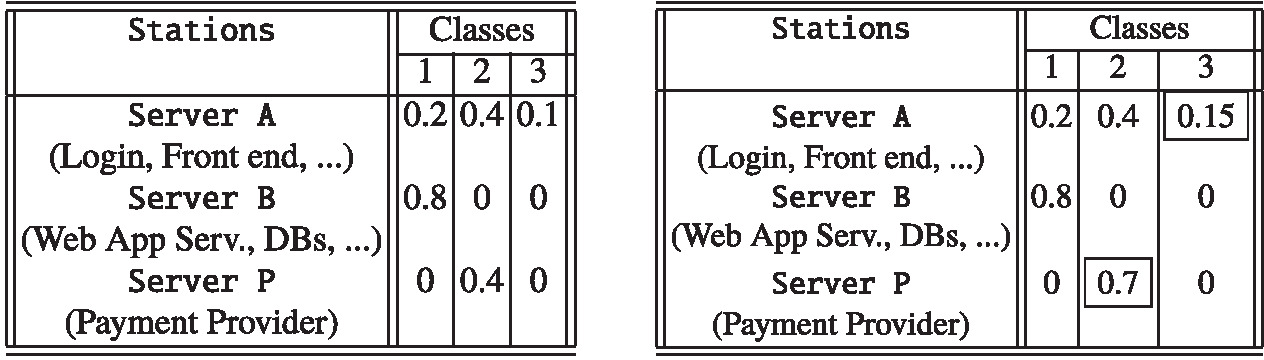
\includegraphics[width=1\linewidth]{figs/average_service_per_job_class_by_node.png}
    \caption{Tempi di servizio medi per classe di job in ogni nodo, nella versione vanilla (sinistra) e con 2FA (destra) \citep{DBLP:books/sp/Serazzi24}}
    \label{fig:average_service_per_job_class_by_node}
\end{figure}

\begin{figure}
    \centering
    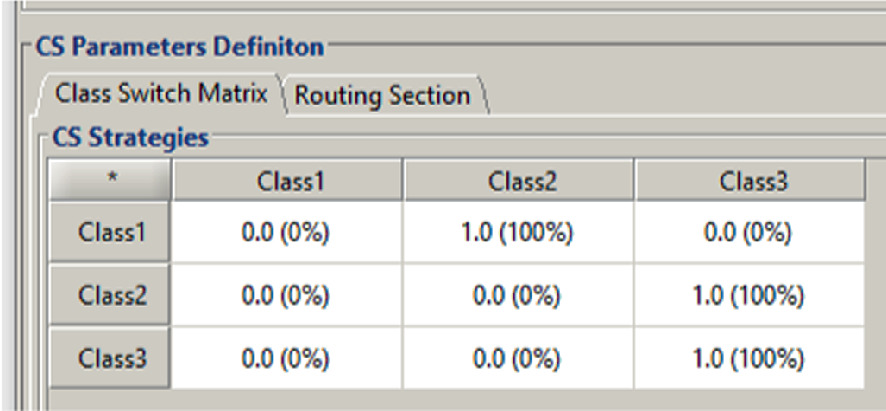
\includegraphics[width=1\linewidth]{figs/routing_matrix.png}
    \caption{Class switch matrix \citep{DBLP:books/sp/Serazzi24}}.
    \label{fig:routing_matrix}
\end{figure}

% Please add the following required packages to your document preamble:
% \usepackage{graphicx}
% \usepackage[table,xcdraw]{xcolor}
% Beamer presentation requires \usepackage{colortbl} instead of \usepackage[table,xcdraw]{xcolor}
\begin{table}[]
\centering
\caption{Routing Matrix per jobs di una certa classe che arrivano in un server. I valori nelle celle implicano una probabilità di routing pari a 1 verso i server specificati e 0 verso tutti gli altri. Il valore EXIT indica l'uscita dal sistema.}
\label{tab:routing-matrix}
\resizebox{\columnwidth}{!}{%
\begin{tabular}{
>{\columncolor[HTML]{FFFFFF}}l |
>{\columncolor[HTML]{FFFFFF}}l |
>{\columncolor[HTML]{FFFFFF}}l |
>{\columncolor[HTML]{FFFFFF}}l |}
\cline{2-4}
{\color[HTML]{222222} }                                                       & {\color[HTML]{222222} class 1}           & {\color[HTML]{222222} class 2}           & {\color[HTML]{222222} class3}        \\ \hline
\multicolumn{1}{|l|}{\cellcolor[HTML]{FFFFFF}{\color[HTML]{222222} Server A}} & {\color[HTML]{222222} \textbf{Server B}} & {\color[HTML]{222222} \textbf{Server P}} & {\color[HTML]{222222} \textbf{EXIT}} \\ \hline
\multicolumn{1}{|l|}{\cellcolor[HTML]{FFFFFF}{\color[HTML]{222222} Server B}} & {\color[HTML]{222222} \textbf{Server A}} & {\color[HTML]{222222} }                  & {\color[HTML]{222222} }              \\ \hline
\multicolumn{1}{|l|}{\cellcolor[HTML]{FFFFFF}{\color[HTML]{222222} Server P}} & {\color[HTML]{222222} }                  & {\color[HTML]{222222} \textbf{Server A}} & {\color[HTML]{222222} }              \\ \hline
\end{tabular}%
}
\end{table}

Le variabili dipendenti sono le seguenti metriche di performance:
\begin{itemize}
    \item Tempo di risposta $T$: detto anche Tempo di Residenza, è l'intervallo di tempo che una richiesta trascorre all'interno di un nodo (o del Sistema) dal momento in cui entra fino al momento in cui esce;
    \item Popolazione $N$: numero di richieste all'interno di un nodo (o nel Sistema);
    \item Throughput $X$: numero di richieste soddisfatte sull'unità di tempo da un nodo (o dal Sistema). 
    \item Utilizzazione $\rho$: proporzione di tempo in cui il nodo è occupato dall'esecuzione delle richieste.
\end{itemize}